\documentclass{beamer}
\usetheme{metropolis}           % Use metropolis theme
\title{Theoretical Time-Complexity of Memory Cache}
\date{\today}
\author{Rasmus Tollund}
\institute{DEIS Junior Club - Aalborg University

\vspace{1cm}
This talk is inspired by \href{http://www.ilikebigbits.com/2014_04_21_myth_of_ram_1.html}{Myth of Ram - by Emil Ernerfeldt}}

\usepackage{graphicx}
\usepackage{tikz}
\usepackage{pgfplots}
\usepackage{array}
\usepackage[linesnumbered,ruled,vlined]{algorithm2e}

% Sources
% http://www.ilikebigbits.com/2014_04_21_myth_of_ram_1.html

\begin{document}

\maketitle
\section{Last Week on Juniour Club}

\begin{frame}{Data Oriented Programming}
\only<1>{
\centering

\includegraphics[width=0.8\textwidth]{resources/nic_talk.pdf}
}
\only<2>{
\begin{columns}[onlytextwidth]
\column{\textwidth}
Key points:
\begin{itemize}
  \item Memory segmented into increasing sized blocks
  \item Larger memory blocks are slower to access
  \item Caching has big impact on performance
\end{itemize}

\vfill
\begin{center}    
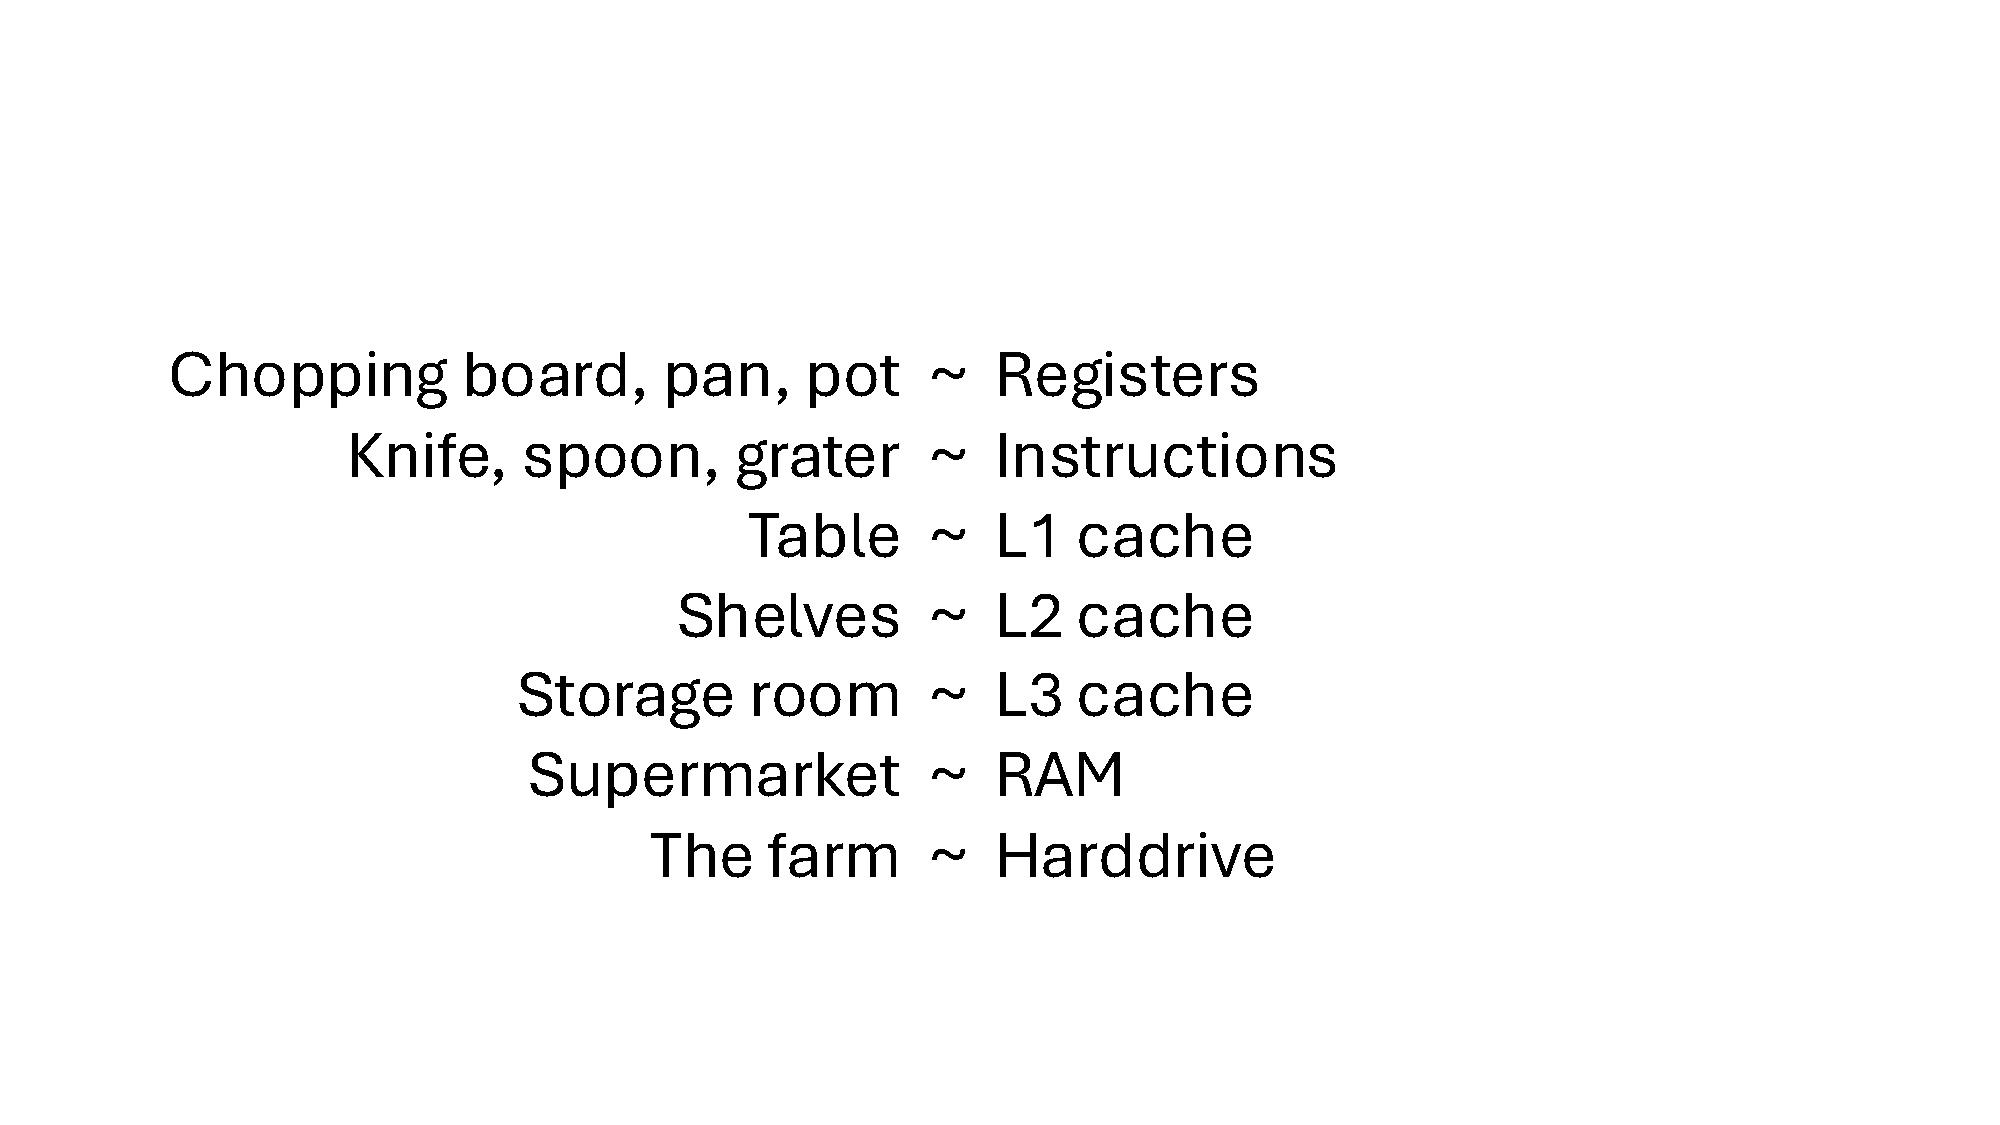
\includegraphics[width=0.3\textwidth]{resources/nic_talk_1.pdf}
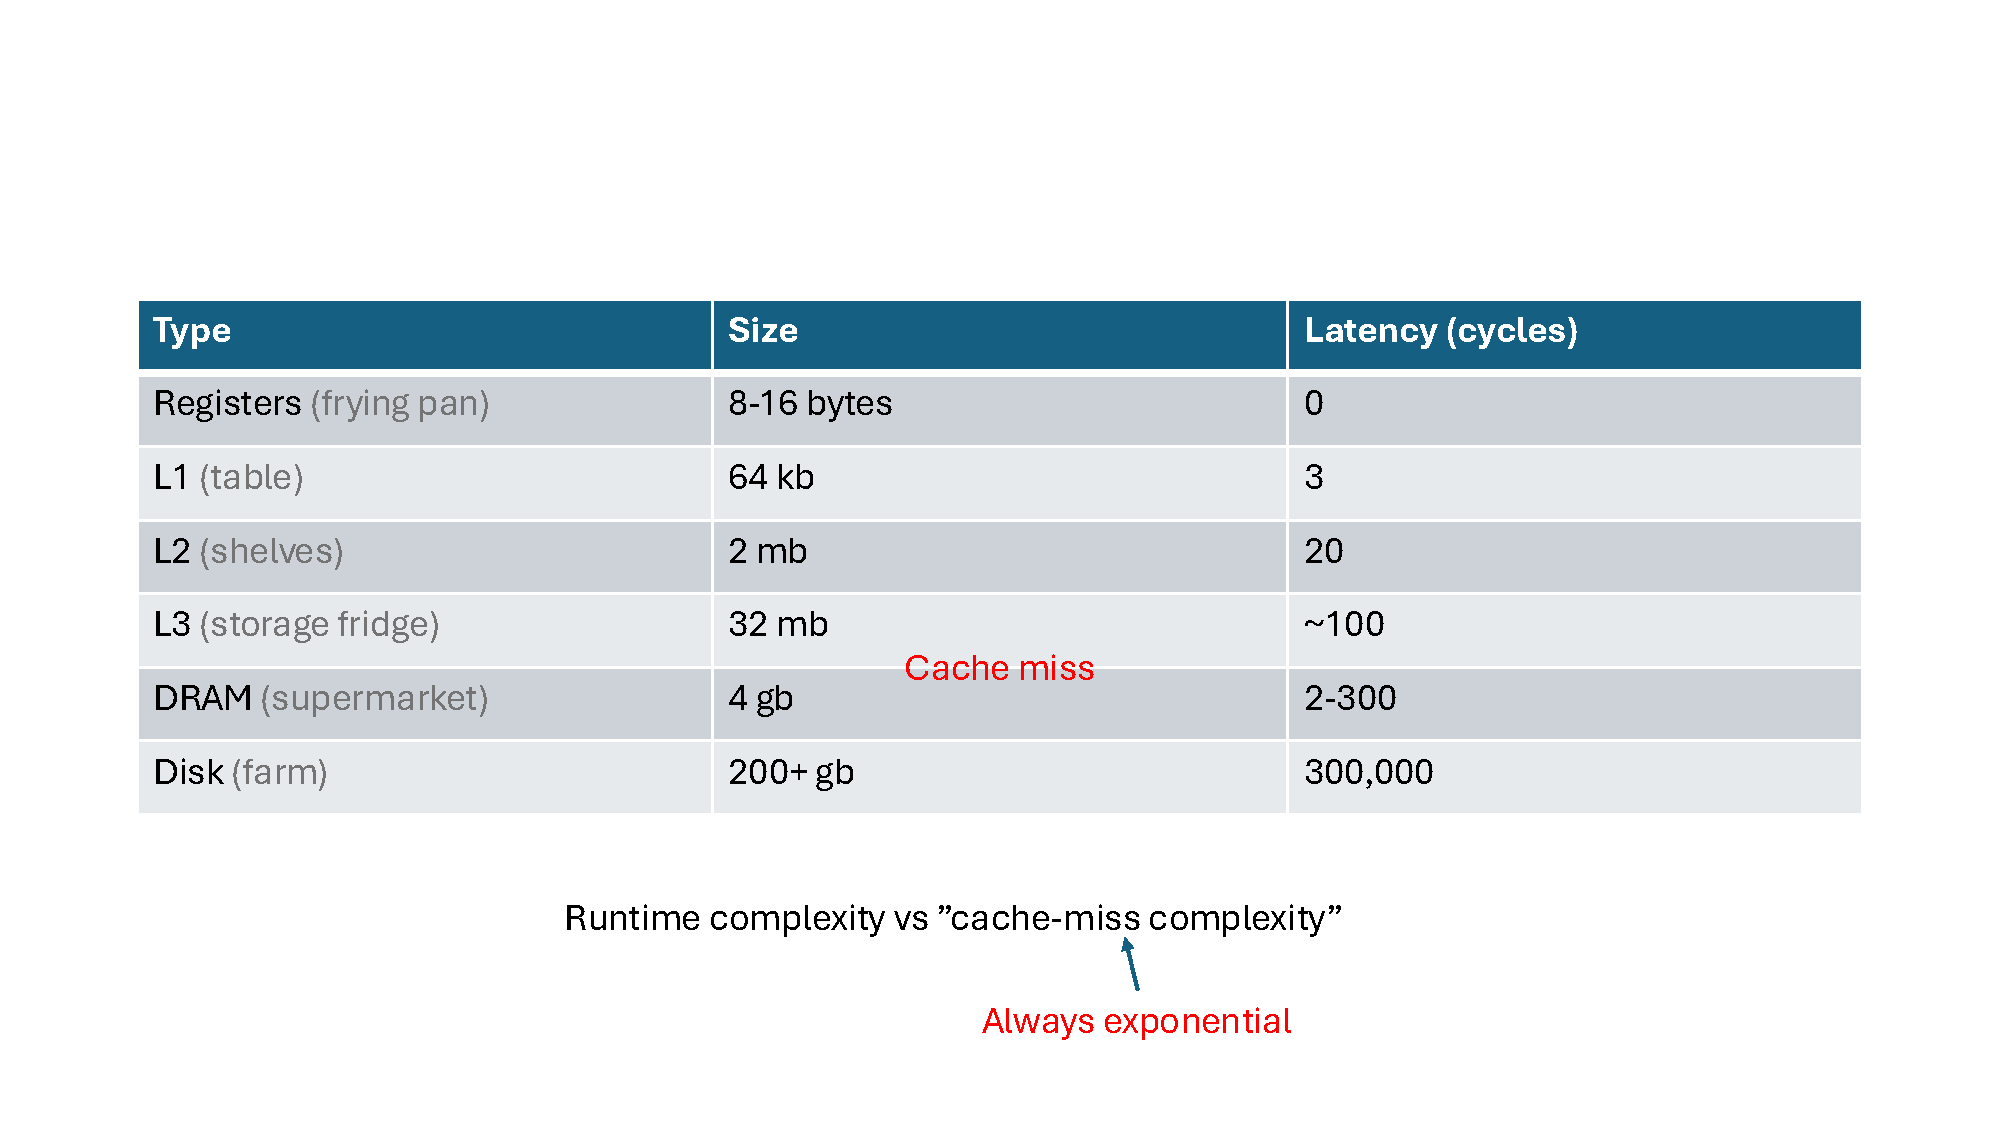
\includegraphics[width=0.3\textwidth]{resources/nic_talk_2.pdf}
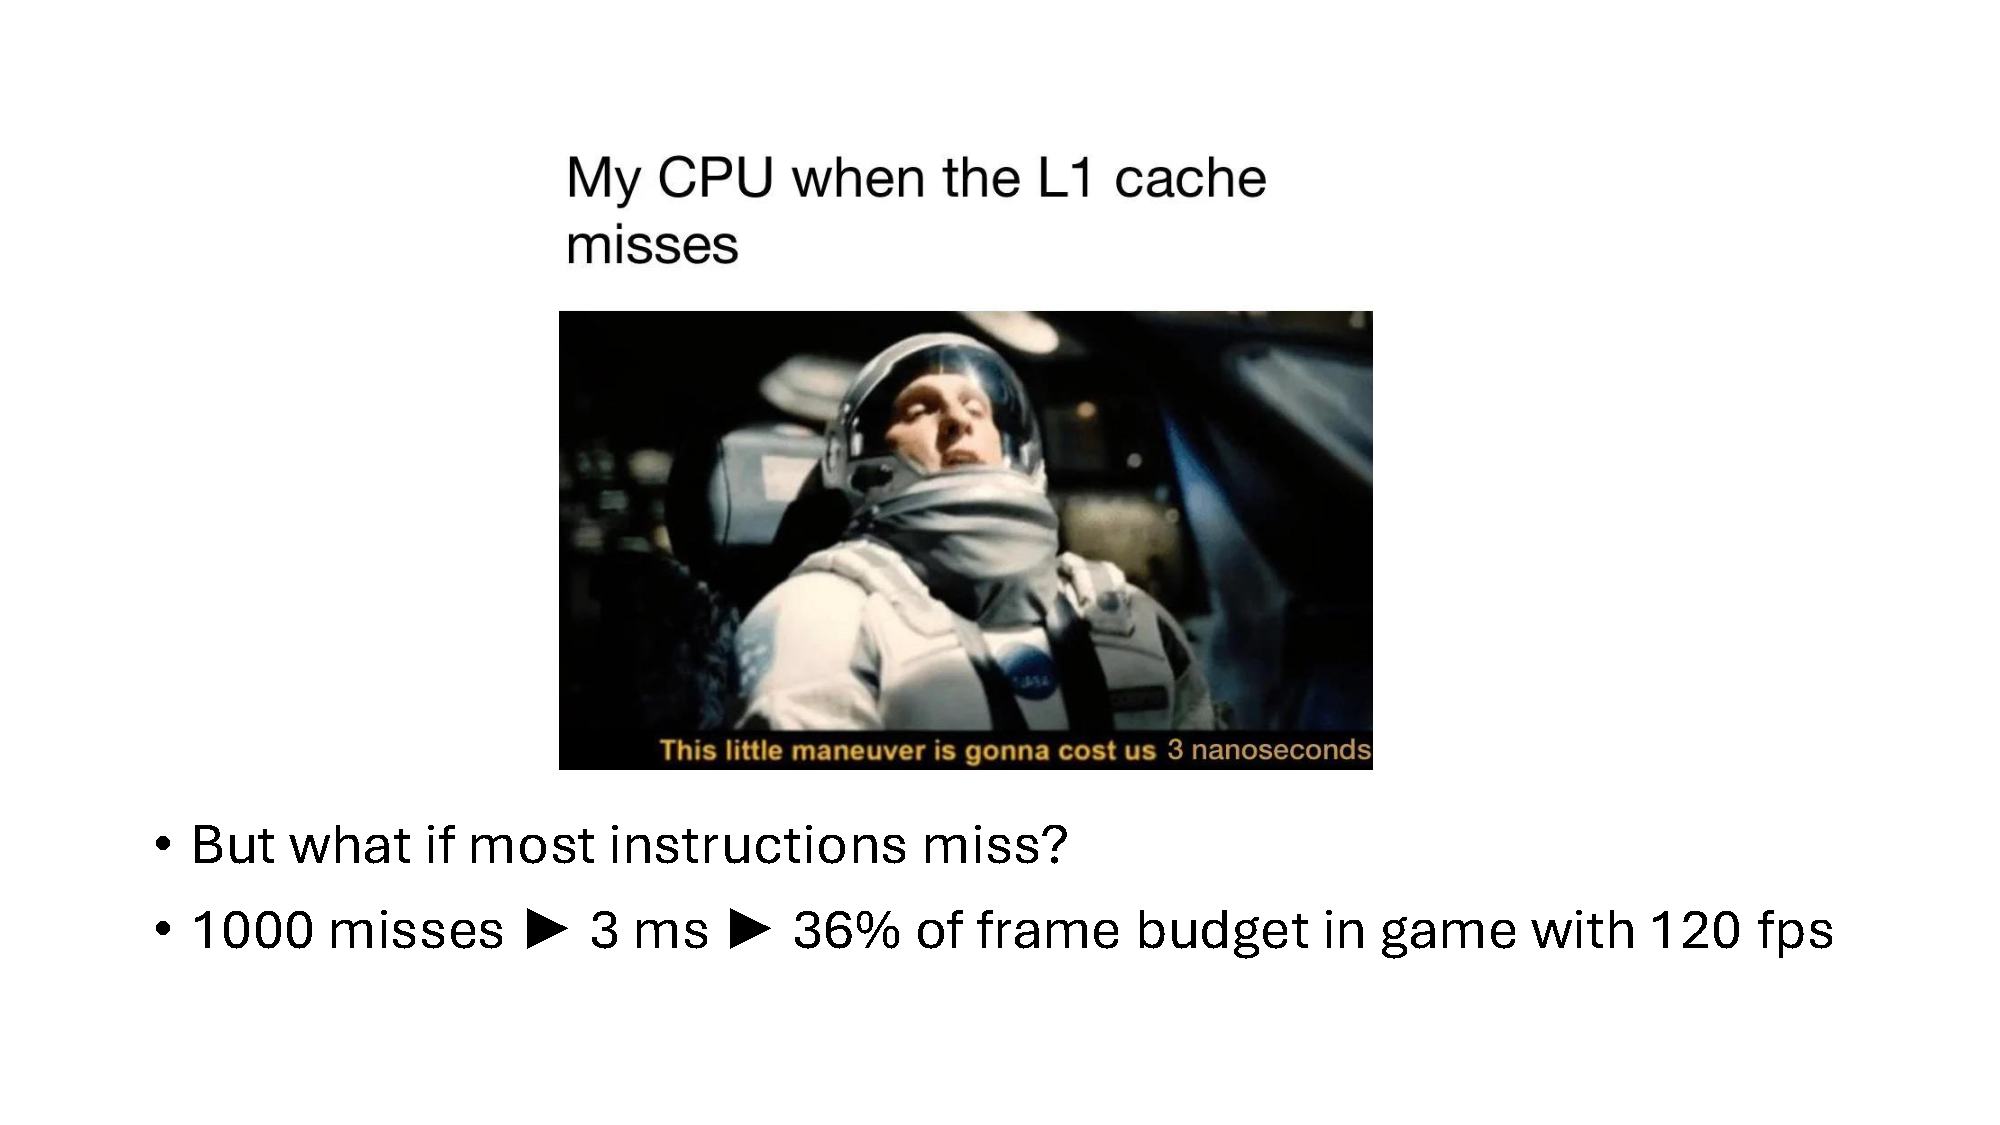
\includegraphics[width=0.3\textwidth]{resources/nic_talk_3.pdf}
\end{center}
\end{columns}
}
\end{frame}


\section{This Week on Junior Club}

\begin{frame}{Latency as a Function of Memory Size}
  \resizebox{\textwidth}{!}{
  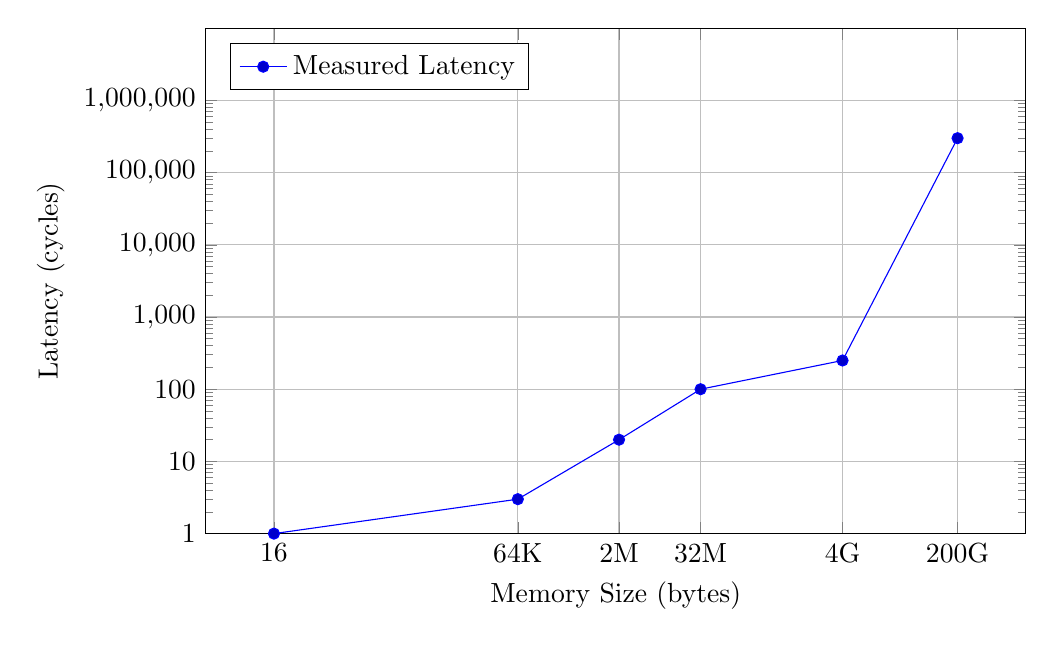
\begin{tikzpicture}
    \begin{axis}[
        xmode=log, ymode=log,
        xlabel={Memory Size (bytes)},
        ylabel={Latency (cycles)},
        xtick={16,64000,2000000,32000000,4000000000,200000000000},
        xticklabels={16,64K,2M,32M,4G,200G},
        ymin=1, ymax=10000000,
        ytick={1,10,100,1000,10000,100000,1000000},
        log ticks with fixed point,
        grid=major,
        width=12cm,
        height=8cm,
        legend pos=north west
    ]
    \addplot coordinates {
        (16, 1)
        (64000, 3)
        (2000000, 20)
        (32000000, 100)
        (4000000000, 250)
        (200000000000, 300000)
    };
    \addlegendentry{Measured Latency}
    \end{axis}
\end{tikzpicture}
}
What is this function?
\end{frame}

\begin{frame}{Caching of Memory}
Memory is cached into levels of increasing size and distance from CPU

\begin{center}
\includegraphics[width=0.5\textwidth,page=6,angle=90,origin=c]{resources/hand_drawings.pdf}
\end{center}
\end{frame}

\begin{frame}{Why not just infinite block of memory?}
Memory must inherently be segmented into levels

\begin{center}
\includegraphics[width=0.4\textwidth,page=5,angle=90,origin=c]{resources/hand_drawings.pdf}
\end{center}

How can the multiplexer decide if an infinite address refers to this memory?
\end{frame}

\begin{frame}{Distance to Memory Based on Size}
Each byte (or bit) has a minimum non-zero size $s$.

\begin{center}
\includegraphics[width=0.6\textwidth,page=4,angle=90,origin=c]{resources/hand_drawings.pdf}
\end{center}
\end{frame}

\begin{frame}{General Distance to Memory in 2 Dimensions}
  In general, in 2 dimensions, the distance access 1 memory unit within $N$ units is proportional to $\sqrt{N}$.


\begin{center}
\includegraphics[width=0.6\textwidth,page=3,angle=90,origin=c]{resources/hand_drawings.pdf}
\end{center}
\end{frame}

\begin{frame}{Computers Are Normally Quite 2-Dimensional}
Computers are very 2-dimensional. At the level of the circut boards, the room, the buildings, distributed over the entire globe.

\begin{center}
\includegraphics[width=0.5\textwidth,page=2,angle=90,origin=c]{resources/hand_drawings.pdf}
\end{center}

\pause
\vspace{-1cm}
But space is 3-dimensional, right?
\end{frame}

\begin{frame}{So How Much is Physically Possible?}
The \emph{Bekenstein Bound} is an upper bound on entropy $(S)$ within a volume enclosed by a radius ($R$) containing mass-energy $E$.
\[
  S \leq \frac{2 \pi k R E}{\hbar c}
\]
Entropy is basically the amount of information, in bits, that exists in the system.
\pause

These are just some constants: $2, \pi, k, \hbar, c$, so
\[
  S \propto RE
\]
\pause
What is the upper bound on mass-energy in a given radius?
\end{frame}

\begin{frame}{A Black Hole}
\begin{center}
\includegraphics[width=0.4\textwidth,page=1,angle=90,origin=c]{resources/hand_drawings.pdf}
\end{center}
\vspace{-0.5cm}

\pause
The \emph{Schwarzchild radius} is the radius defining the event horizon of a black hole.
\[
  R_s = \frac{2 G M}{c^2}
\]
\pause
Again, some constants: $2, G, c$, so
\[
  R_s \propto M \quad\text{and thus}\quad M\propto R_s
\]
\end{frame}

\begin{frame}{Upper Bound on Entropy}
By applying this in the Bekenstein bound, we get
\[
  S \propto R^2.
\]
Thus, the maximum amount of information in a sphere of radius $R$ is proportional to $R^2$.


\begin{center}
  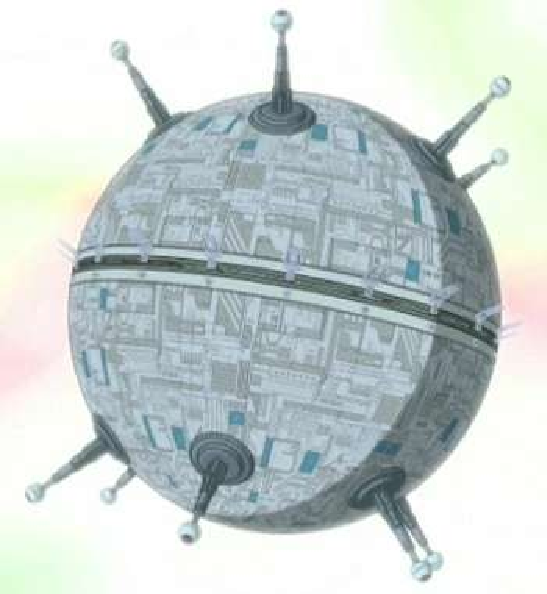
\includegraphics[width=0.4\textwidth]{resources/Infosphere.pdf}
\end{center}
\end{frame}


\begin{frame}{Memory Access is $\mathcal{O}(\sqrt{N})$}
  Since we are limited by the speed of light, the time to to extract data from $N$ bits is proportional to the radius, and thus we will need $\mathcal{O}(\sqrt{N})$ time.


\begin{center}
  \includegraphics[width=0.45\textwidth,page=4,angle=90,origin=c, clip,trim={3cm 0 0 0}]{resources/hand_drawings.pdf}
\end{center}

\vspace{-2cm}
\[
  \text{access time} \geq c s \sqrt{N}
\]
\end{frame}

\begin{frame}{Does this match empirical data?}
  How does this fit into the graph we saw earlier?

  \resizebox{\textwidth}{!}{
  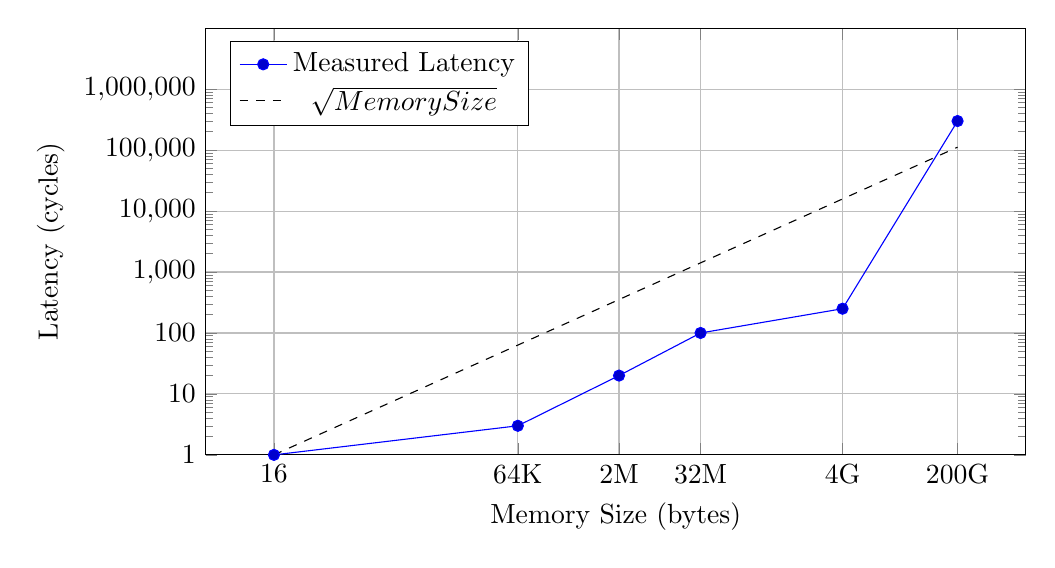
\begin{tikzpicture}
    \begin{axis}[
        xmode=log, ymode=log,
        xlabel={Memory Size (bytes)},
        ylabel={Latency (cycles)},
        xtick={16,64000,2000000,32000000,4000000000,200000000000},
        xticklabels={16,64K,2M,32M,4G,200G},
        ymin=1, ymax=10000000,
        ytick={1,10,100,1000,10000,100000,1000000},
        log ticks with fixed point,
        grid=major,
        width=12cm,
        height=7cm,
        legend pos=north west
    ]
    \addplot coordinates {
        (16, 1)
        (64000, 3)
        (2000000, 20)
        (32000000, 100)
        (4000000000, 250)
        (200000000000, 300000)
    };
    \addlegendentry{Measured Latency}
    
    \addplot[domain=16:200000000000, samples=100, dashed] {sqrt(x/16)};
    \addlegendentry{$\sqrt{\text{Memory Size}}$}
    \end{axis}
\end{tikzpicture}
}

  \pause
  What does this mean for asymptotic analysis of algorithms?
\end{frame}

\section*{Applying The New Model}

\begin{frame}{Time-Complexity of Search in Linked List}
Traditionally, searching a linked list is $\Theta(N)$ time-complexity. However, all lookups are random access. Thus, the complexity in the new model, is actually $\Theta(N \sqrt{N})$.

\pause
\begin{center}
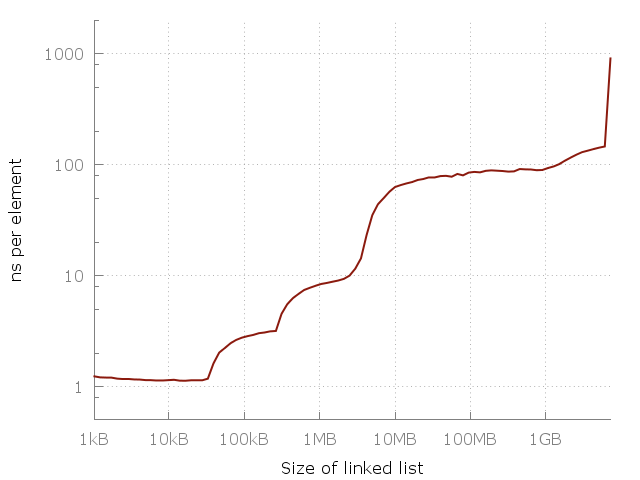
\includegraphics[width=0.7\textwidth]{resources/linked_list.png}
\end{center}
\vspace{-1cm}
\end{frame}

\begin{frame}{Time-Complexity of Bubble Sort}
Assume all memory access is random. Notice, not a tight bound.
\begin{algorithm}[H]
\DontPrintSemicolon
\SetKwInOut{Input}{Input}
\SetKwInOut{Output}{Output}

\Input{Array $A$ of length $N$}
\Output{Sorted array $A$ in ascending order}

\For(\tcp*[f]{$\mathcal{O}(\sqrt{\log N})$}){$i \gets 0$ \textbf{to} $N-1$ } {
  \For(\tcp*[f]{$\mathcal{O}(\sqrt{\log N})$}){$j \gets 0$ \textbf{to} $N-i-2$} {
      \If(\tcp*[f]{$\mathcal{O}(\sqrt{N})$}){$A[j] > A[j+1]$} {
        Swap $A[j]$ and $A[j+1]$ \tcp*[r]{$\mathcal{O}(\sqrt{N})$}
      }
    }
}
\caption{Bubble Sort}
\end{algorithm}
\pause
Time-complexity
\begin{align*}
  \mathcal{O}(N) \cdot \left(\mathcal{O}(\sqrt{\log N}) + \mathcal{O}(N) \cdot \left( \mathcal{O}(\sqrt{\log N}) + \mathcal{O}(\sqrt{N}) + \mathcal{O}(\sqrt{N})  \right) \right) \\ = \mathcal{O}(N^2 \sqrt(N))
\end{align*}
\pause
Normally: $\Theta(N^2)$
\end{frame}


\begin{frame}{When does this matter?}
If we assume all memory access is random, this basically means:
\begin{block}{}
  Let algorithm have normal time-complexity $\Theta(t(n))$ and space-complexity (including input) $\Theta(s(n))$. The new time-complexity is $\mathcal{O}(t(n)\cdot \sqrt{s(n)})$
\end{block}
\pause

\vfill
\begin{tabular}{|c|>{\raggedright}p{2.5cm}|>{\raggedright}p{2.5cm}|>{\raggedright}p{2.5cm}|} \hline & \textbf{Normal~Time \mbox{Complexity}} & \textbf{Space \mbox{Complexity}} & \textbf{New~Time \mbox{Complexity}} \tabularnewline
    \hline
    Alg. 1 & $\Theta(n^2)$ & $\Theta(n^2)$ & $\mathcal{O}(n^3)$ \tabularnewline
    \hline
    Alg. 2 & $\Theta(n^2 \log n)$ & $\Theta(n)$ & $\mathcal{O}(n^2 \sqrt{n} \log n)$ \tabularnewline
    \hline
\end{tabular}
\end{frame}

\begin{frame}{So Does This Help With Considering Cache?}
Not really...
\pause

Assuming all memory access is random gives us an upper bound, but it does not help us distinguish proper cache usage.
\end{frame}

\begin{frame}{Not All Memory Access is Random}
We know that not all memory access is random. Let us consider linear search through an array of $N$ elements.

How can we analyze the complexity of this algorithm?

\begin{center}
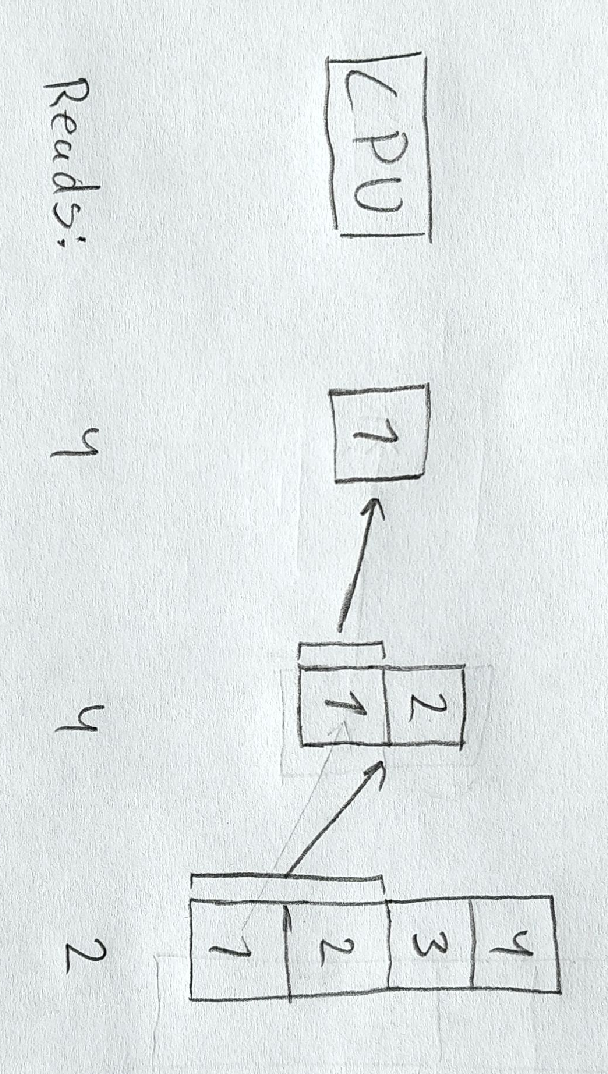
\includegraphics[width=0.4\textwidth,page=1,angle=90,origin=c]{resources/hand_drawings2.pdf}
\end{center}

\end{frame}

\begin{frame}{Generalizing Cache Layout}
Let $S_i$ be the size of the $i$'th cache $L_i$. Let us assume that filling $L_i$ with $S_i$ values of $L_{i+1}$ can be done in time $\Theta(\sqrt{S_{i+1}})$.

\begin{center}
\includegraphics[width=0.4\textwidth,page=2,angle=90,origin=c]{resources/hand_drawings2.pdf}
\end{center}
\vspace{-3cm}

\pause
How big should $L_i$ be?
\end{frame}

\begin{frame}{Memory Accesses to Caches}
  In linear search, for each unique chunk in $L_i$, $L_{i+1}$ will read it $\lceil \frac{S_i}{S_{i-1}} \rceil$ times. There are $\lceil \frac{N}{S_i} \rceil$ unique chunks. Thus, $L_i$ receives $\lceil \frac{S_i}{S_{i-1}} \rceil \lceil \frac{N}{S_i} \rceil \approx \frac{N}{S_{i-1}}$ reads. Each has the complexity $\Theta(\sqrt{S_i})$.

\vfill
\pause
The total number of reads in an $N$ array will be
\[
  \sum^{k}_{i=1} \frac{N}{S_{i-1}} \Theta(\sqrt{S_i}),
\]
where $k=\min\{i\in \mathbb{N} \mid N \leq S_i\}$.

\end{frame}

\begin{frame}{Which Caching Size Strategy to Use}
Let us try with $S_i = i$. This yields
\[
  \sum^N_{i=2} \frac{N}{i-1} \Theta(\sqrt{i}) = N \sum^N_{i=2} \Theta\left(\frac{1}{\sqrt{i}}\right) = \Theta(N\sqrt{N}).
\]

\pause
What about $S_i = 2^i$?
\[
  \sum^{\log N}_{i=1} \frac{N}{2^{i-1}} \Theta(\sqrt{2^i}) = N \underbrace{\sum^{\log N}_{i=1} \frac{\Theta(\sqrt{2^i})}{2^{i-1}}}_{\text{bounded}} = \Theta(N)
\]

\pause
Cool! Assuming exponentially increasing cache sizes, optimal locality usage is actually (amortized) constant access.
\end{frame}

\begin{frame}{Merge Sort Vs. Heap Sort}
Merge sort uses optimal memory locality, thus $\Theta(n\log n)$. Heap sort is mostly random access, thus $\Theta(n\log n \sqrt{n})$.


\end{frame}


% \begin{frame}{Cache-Oblivious Model of Computation}
% Another model, is the cache-oblivious model of computation. Basically, the algortihm is oblivious to the size of the cache, but the complexity is in how many cache-misses occurs.
% \end{frame}

\begin{frame}{Conclusion}
\begin{itemize}
  \item Due to physics, random access is $\Theta(\sqrt{N})$
  \item With careful analysis, we can get cache-aware time-complexity
  \item Optimal locality usage is amortized constant time
\end{itemize}
\end{frame}



\end{document}
